\documentclass[10pt]{article}

\usepackage{amsmath}
\usepackage{amssymb}
\usepackage{mathtools}
\usepackage{array}
\usepackage{booktabs}
\usepackage[margin=1in]{geometry}
\usepackage{graphicx}

\newcommand{\np}{\vfill\newpage}

\begin{document}

\pagenumbering{gobble}

%This creates the title of the document.
\begin{center}
    \LARGE{Aphid Management for Apple Growers} \\
    \vspace{0.15in} 
    \large{The Bilbies: Zane Billings, Nicholas Ruby, \& Prem Kumar Subbukutti} \\
    \large{MATH 430: Mathematical Modeling} \\
    \large{20 February, 2019} \\
    \vspace{0.25in}
\end{center}

%The table of contents goes here.

\tableofcontents
\np

\pagenumbering{arabic}

\section{Technical Report}

\subsection{Model and Parameters}

In order to model the IPM system for the populations of aphids and ladybugs, we have the following system of differential equations.

\begin{align}
\dot{A} &= rA - \alpha A L \label{eq:basicA}\\
\dot{L} &= -cL + \beta A L \label{eq:basicL}
\end{align}

The aphid population, in millions, is represented as \(A\) and \(L\) is the population of ladybugs in tens of thousands, both in terms of time \(t\). The simple Lotka-Volterra model we are using assumes a natural growth rate for the aphid population, represented by \(r\), and a natural decay rate for the ladybug population, represented as \(c\). Note that both \(r\) and \(c\) are positive percentages; the coefficient \(r\) is positive in the model to represent growth, while the \(c\) parameter is negative to represent the decline in the ladybug population over time. 

The term in both equations containing \(AL\) is the ``handshake'' parameter of the model, representing the possible interactions between the two populations. The term \(\beta\) represents the proportion of interactions in which a predator can kill prey organisms (and thus the population can grow due to energy obtained by the predator), and likewise, \(\alpha\) represents the proportion of interactions fatal for prey organisms. Both of these parameters combine an encounter rate and a ``predator success'' rate measuring the efficiency of the predators at hunting.

\subsection{Equilibria of the Basic Model}

By setting \(\dot{A}\) and \(\dot{L}\) equal to zero in equations \ref{eq:basicA} and \ref{eq:basicL} above, the equilibria, or fixed points, of the system can be found. Solving in Mathematica, we obtain the equilibrium points 
\[(0,0) \ \mathrm{and} \ \left( \frac{c}{\beta},\frac{r}{\alpha} \right),\]
both points of the form \((A,L)\). Thus, these two points will determine what happens given any initial condition for the two populations. In order to determine the stability of the equilibria, we apply both the nullcline method as well as a linearization method near the equilibria to determine the stability of the equilibria using the eigenvalue method.

Examining the nullcline plot in Figure \ref{fig:basicmodelnullcline}, we see saddle behavior at the equilibrium point \( (0,0) \), and center behavior about the other equilibrium point, which with the given set of parameters can be approximately calculated as the point $(1.25,1.62)$. The nullcline approach indicates that a population of aphids, regardless of size, will grow without bound without ladybugs present, and without aphids present, a ladybug population of any size will decay to zero over time. Any initial population of aphids and ladybugs will remain in a limit cycle about the point $(1.25,1.62)$. Note that all nullcline plots are found at the end of the technical report.

To obtain a more analytic determination of stability of the equilibria, we can linearize the system about the equilibria of interest using the Jacobian matrix of the system. The Jacobian matrix evaluated at a point is defined as 
\[ J_{A*,L*} = 
\begin{bmatrix}
\frac{\partial \dot{A}}{\partial A} & \frac{\partial \dot{A}}{\partial L} \\[1ex]
\frac{\partial \dot{L}}{\partial A} & \frac{\partial \dot{L}}{\partial L}
\end{bmatrix}_{(A=A*,L=L*)}, \]

which for the given system can be calculated as

\[ J_{A*,L*} = 
\begin{bmatrix}
r-L\alpha & -A\alpha \\[1ex]
L\beta & -c+A\beta
\end{bmatrix}_{(A=A*,L=L*)}. \]

Evaluating with the provided set of parameters,

\[ \begin{cases}
r = 0.21 \\
c = 0.10 \\
\alpha =0.13  \\
\beta = 0.08,
\end{cases} 
\]

we obtain the Jacobian matrices

\[ J_{(0,0)} = J_1 =  
\begin{bmatrix}
0.21 & 0 \\[1ex]
0 & -0.1
\end{bmatrix} \
\mathrm{ and } \
J_{\left( \frac{0.10}{0.08},\frac{0.21}{0.13} \right)} = J_2 \approx
\begin{bmatrix}
 0 & -0.16 \\[1ex]
 0.13 & 0
\end{bmatrix}. \]

The eigenvalues of the matrices can be approximated by
\[
\begin{cases}
J_1: \ \lambda = \{-0.10, \ 0.21\} \\
J_2: \ \lambda = \{\pm 0.14i\}
\end{cases}
\]

The eigenvalues of \(J_1\) correspond to a saddle point, and the eigenvalues of \(J_2\) correspond to a center point~\cite{TDplane}. Thus, we see that the equilibrium point (0,0) is an unstable equilibrium and the nontrivial equilibrium point is stable. The nontrivial equilibrium is not stable in the sense that all trajectories will collapse into the same point over time, but all trajectories will form a limit cycle. The findings using the linearization method match the heuristic findings from the nullcline analysis.

While the basic model provides a solid basis for predicting ideal IPM strategies, one particular case is illogical in light of the biological situation underpinning the mathematics. Under the assumptions of the Lotka-Volterra model as stated, if no ladybugs are introduced then the aphid population will grow without bound, which is clearly impossible. Thus, we introduce a logistic term into the model to more accurately reflect the situation.

\subsection{Adjustments for Carrying Capacity}

The Lotka-Volterra model can be easily modified to account for carrying capacity of the aphid population~\cite{beltrami}. The ladybug population is already intrinsically limited by the size of the aphid population, so a carrying capacity only needs to be introduced to the aphid population equation. Adjusting the model to include a logistic term, we obtain the following modified system.

\begin{align}
\dot{A} &= rA\left( 1-\frac{A}{k} \right) - \alpha A L \label{eq:logA}\\
\dot{L} &= -cL + \beta A L \label{eq:logL}
\end{align}

In the updated system, \(k\) represents the carrying capacity of the aphid population. Four different carrying capacities were considered: 2, 3, 5, and 10 (all in millions). Again, Mathematica was used to symbolically solve for the equilibrium values by setting \(\dot{A}\) and \(\dot{L}\) equal to 0. For this system, we obtain the trivial equilibrium again, as well as two more equilibria:

\[(k,0) \ \mathrm{and} \ \left (\frac{c}{\beta}, \frac{-r(c-k\beta)}{k\alpha\beta}\right).\]

Using the nullcline approach for a variety of \(k\) values (as listed above), all models show the same behavior. The nullcline plots used for analysis appear below in Figure \ref{fig:logmodelnullcline}.

Since all cases appear to have the same value, we chose the case \(k=3\) as the parameter for further calculations. This system was additionally linearized around each of the equilibrium points, and the respective eigenvalues were computed. Letting \(J_{(A*,L*)}\) be the Jacobian for the system, evaluated at the equilibrium point \((A*,L*)\), we have the eigenvalues

\[\begin{cases}
J_{ (0,0) }: \lambda = \{-0.21,0.10\} \\
J_{ (k,0) }: \lambda = \{-0.21,0.7\} \\
J_{ ( \frac{c}{\beta} ,\frac{-r(c-k\beta)}{k\alpha\beta}) }: \lambda \approx \{ -0.044 \pm 0.102i \}
\end{cases}
\]

Thus, the equilibria are, respectively, two saddle points, and a spiral sink~\cite{TDplane}. These equilibria represent different system behavior than the basic Lotka-Volterra equations. Here, we see that without introducing ladybugs (a predator population), the aphid population will grow to its carrying capacity and cease growing. Again however, ladybugs will suffer a catastrophe and fall to zero if there are no aphids. The equilibria \((0,0)\) and \((k,0)\) are both unstable, and if both populations coexist, they will fall away from these equilibria.

However, the spiral sink at the nontrivial equilibrium is asymptotically stable, and any initial condition where both ladybugs and aphids are present will form a trajectory toward this equilibrium over time.

\subsection{Use of Pesticides}

Assuming pesticides are sprayed at a constant rate which kills insects at a rate \(f\) without discriminating against ladybugs or aphids, we can modify the basic system again to consider the effects of pesticide use and IPM in tandem. We obtain the following system.

\begin{align}
\dot{A} &= rA - \alpha A L -fA \label{eq:pesticideA}\\
\dot{L} &= -cL + \beta A L -fL \label{eq:pesticideL}
\end{align}

Solving for the equilibria, we obtain the trivial equilibrium, as well as a modified nontrivial equilibrium point, namely
\[ \left( \frac{c+f}{\beta}, \frac{r-f}{\alpha} \right). \]

Assuming \(f\leq \mathrm{min}\{r,c\}\), nullcline analysis for a variety of \(f\) values (\(f = 0.01,0.02,0.05,0.1\)) shows that the nontrivial equilibrium remains a center point. However, the nullclines additionally suggest that higher values of \(f\) tend to increase the size of the aphid population relative to the ladybug population. The nullcline plots for the different values of \(f\) are shown in Figure \ref{fig:pesticidemodelnullcline}.

Using the linearization method as with the other model formulations to find eigenvalues for the equilibrium points, we find that, as with the basic Lotka-Volterra model, the trivial equilibrium is a saddle point, and the nontrivial equilibrium is a center point. As the stability of the equilibria is unchanged in this formulation of the model, the eigenvalues are less important to the results found by the pesticide/IPM tandem model.

Overall the model predicts that the combined use of IPM and pesticide spraying likely leads to a larger pest (aphid) population than IPM alone, as visualized by the nullcline plots.

\np

\begin{figure}[h]
\centering
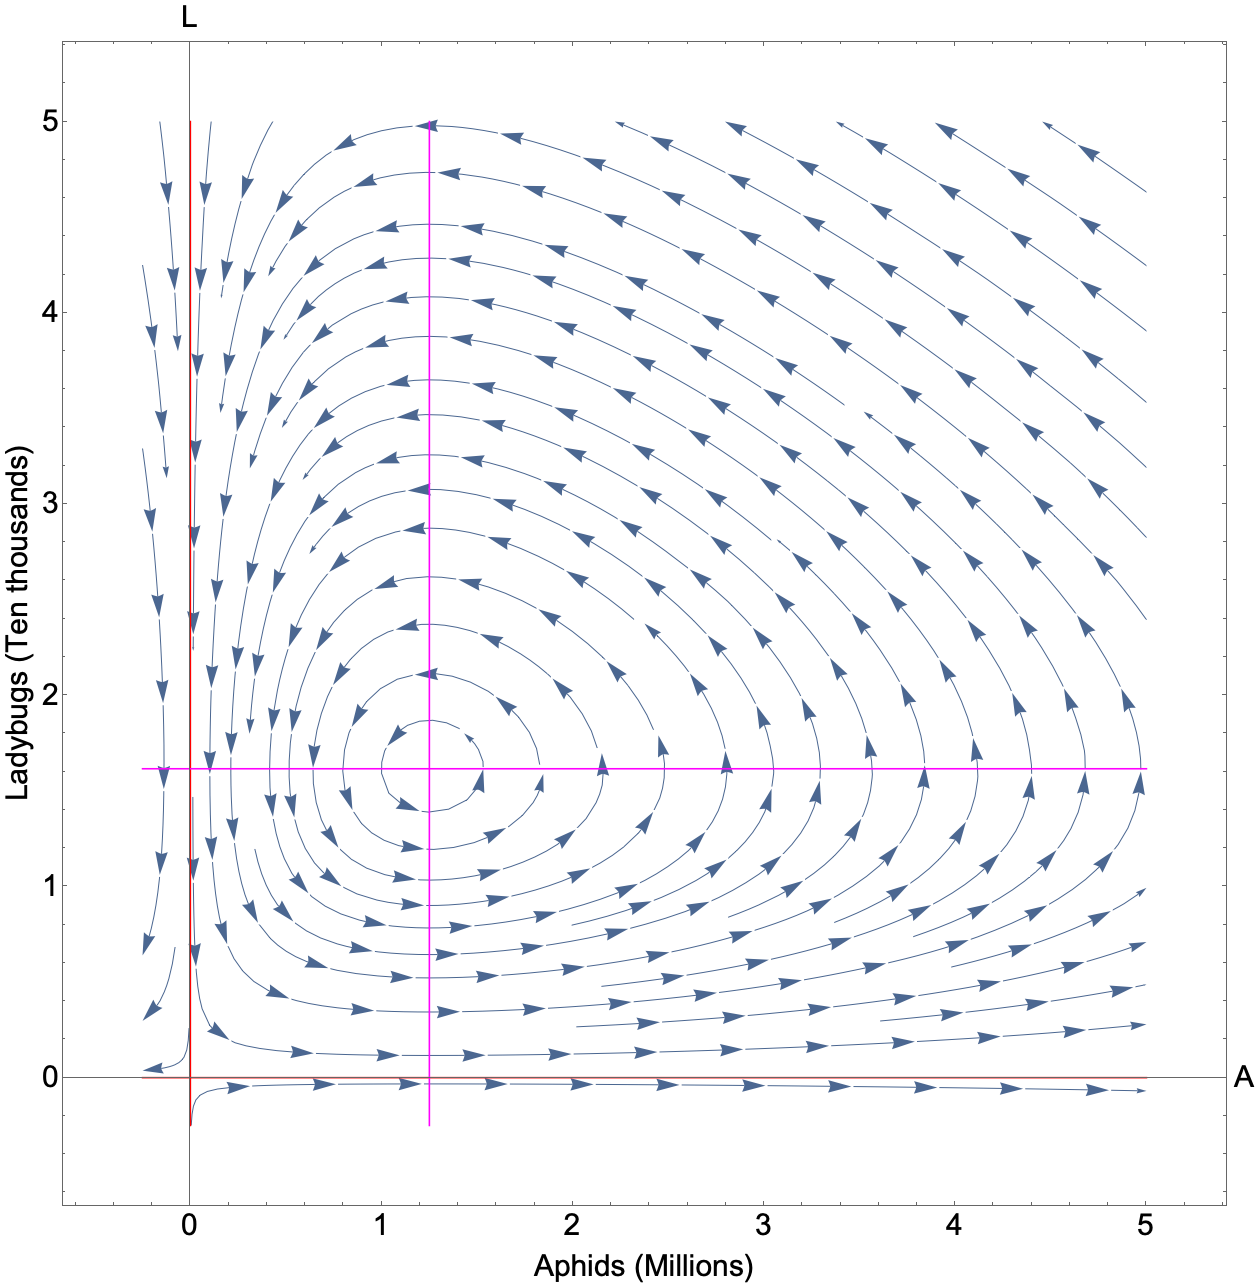
\includegraphics[width=0.9\textwidth]{basic_model_stream_plot.png}
\caption{A vector plot showing the behavior of the derivatives in the first quadrant. The red lines represent the nullclines from the trivial equilibrium and the pink lines represent the nullclines from the nontrivial equilibrium. Note the cyclical motion around the equilibrium at the intersection of the pink nullclines.}
\label{fig:basicmodelnullcline}
\end{figure}

\np

\begin{figure}[h]
	\centering
	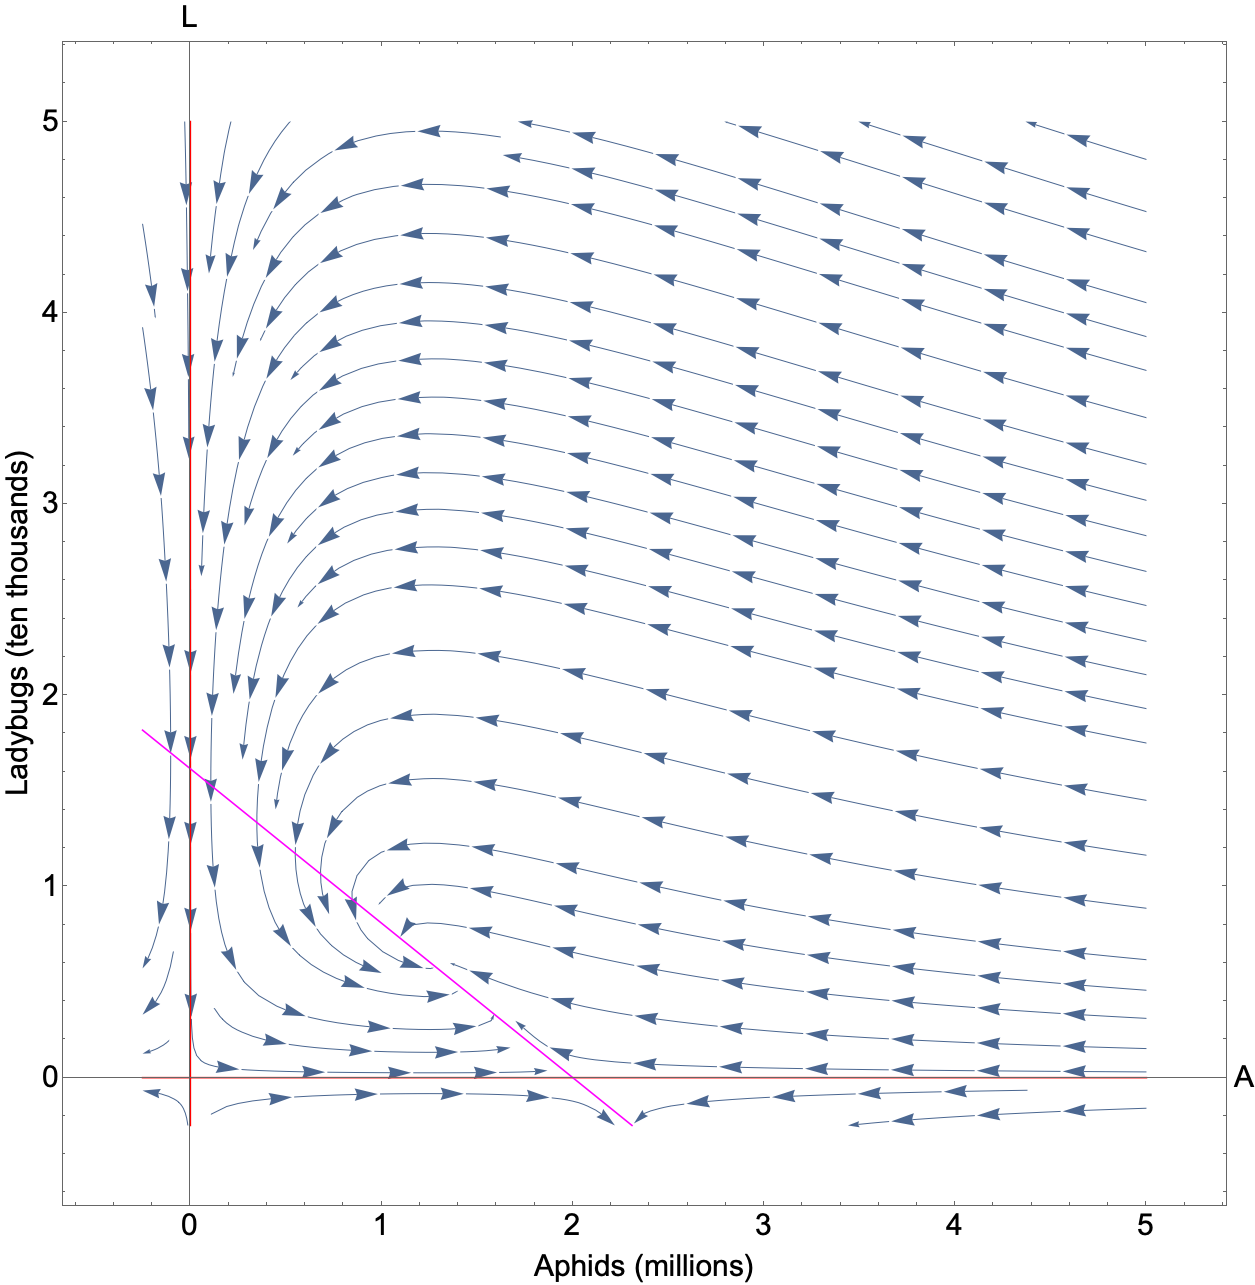
\includegraphics[width=0.45\textwidth]{log_model_nullclines_k2.png}
	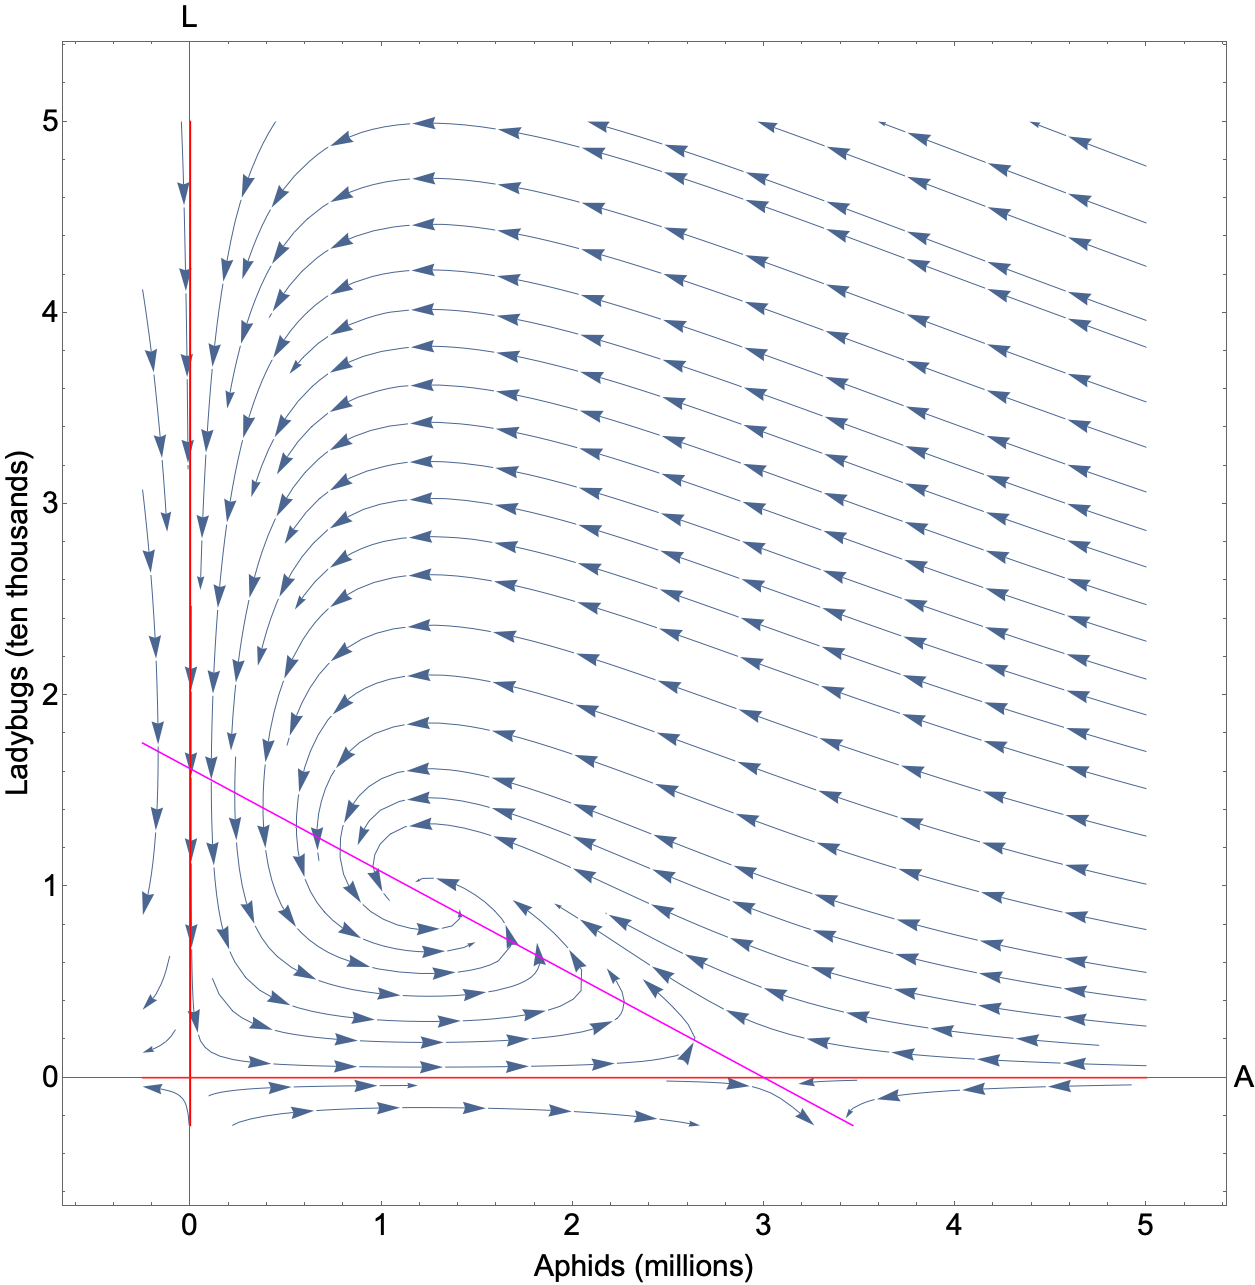
\includegraphics[width=0.45\textwidth]{log_model_nullclines_k3.png} \\ [1ex]
	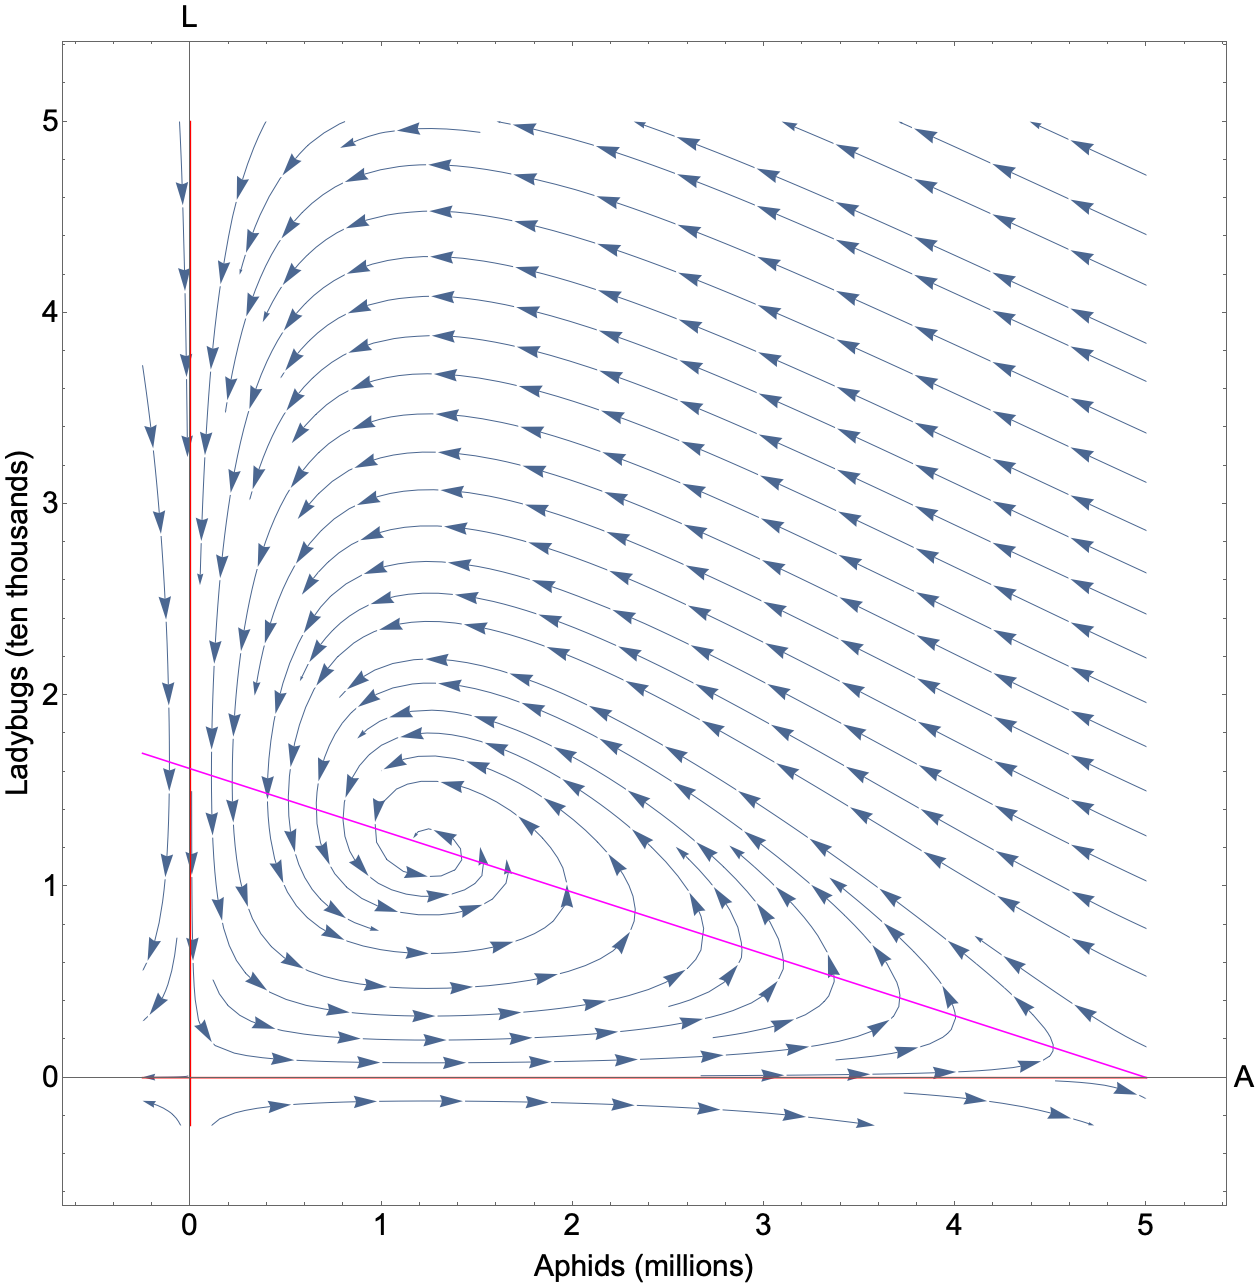
\includegraphics[width=0.45\textwidth]{log_model_nullclines_k5.png}
	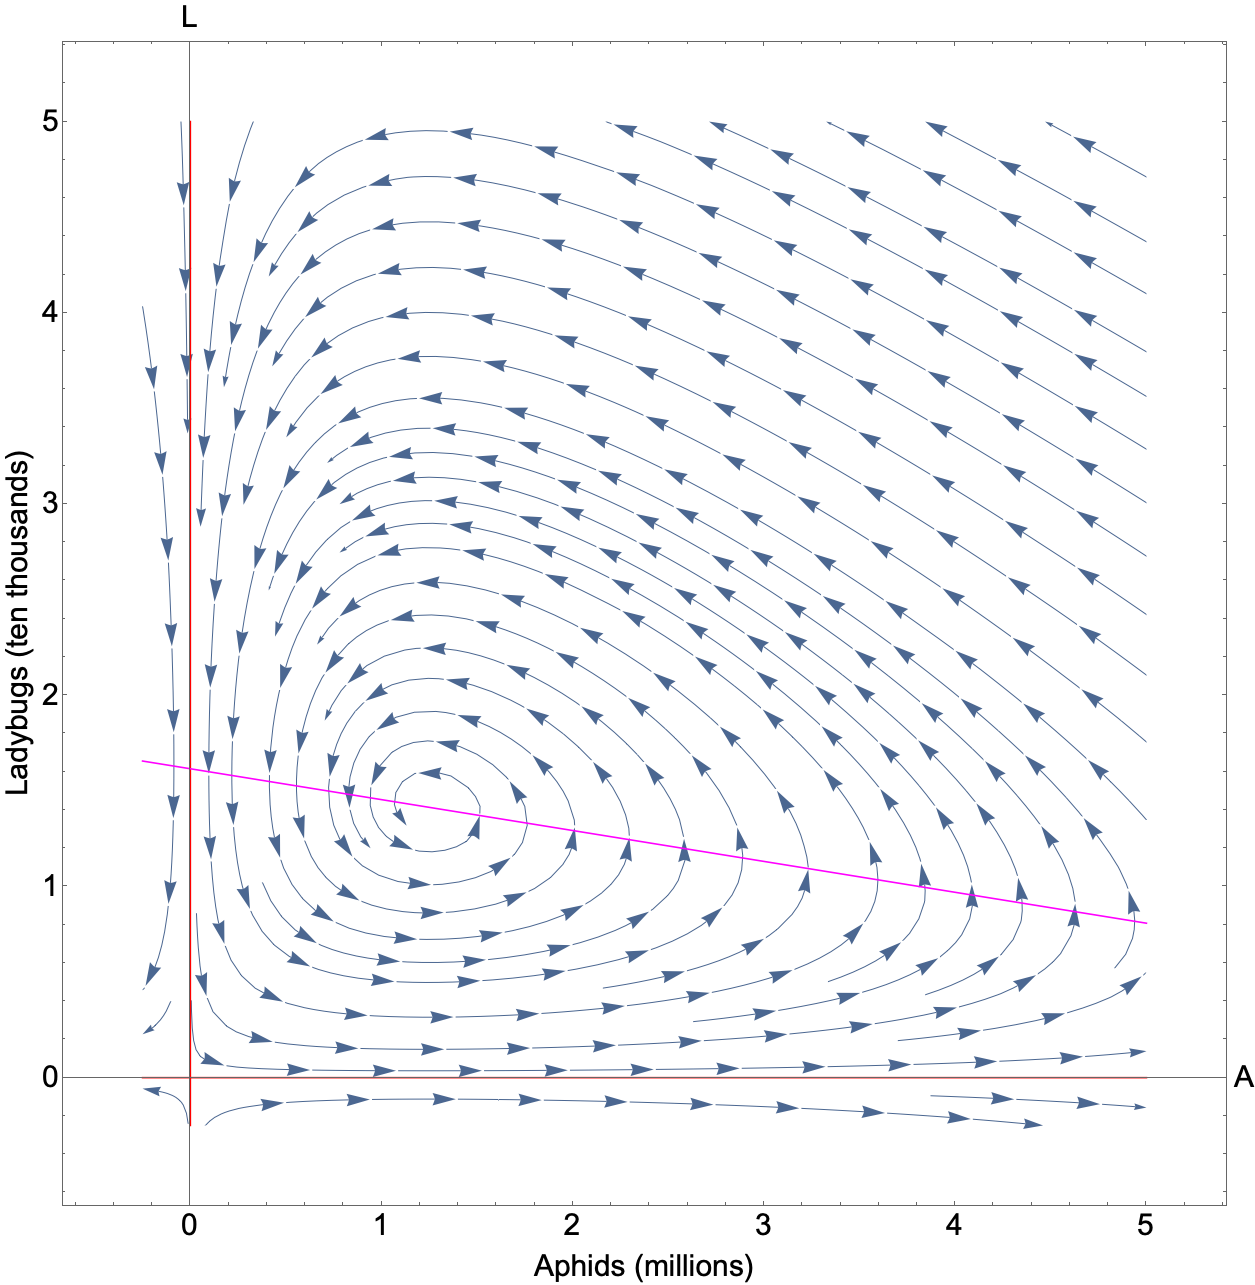
\includegraphics[width=0.45\textwidth]{log_model_nullclines_k10.png}
	\caption{Clockwise from top left: \( k = 2, \ 3, \ 5, \ 10 \). All nullclines show the same behavior of approaching the nontrivial equilibrium point.}
	\label{fig:logmodelnullcline}
\end{figure}

\np

\begin{figure}[h]
	\centering
	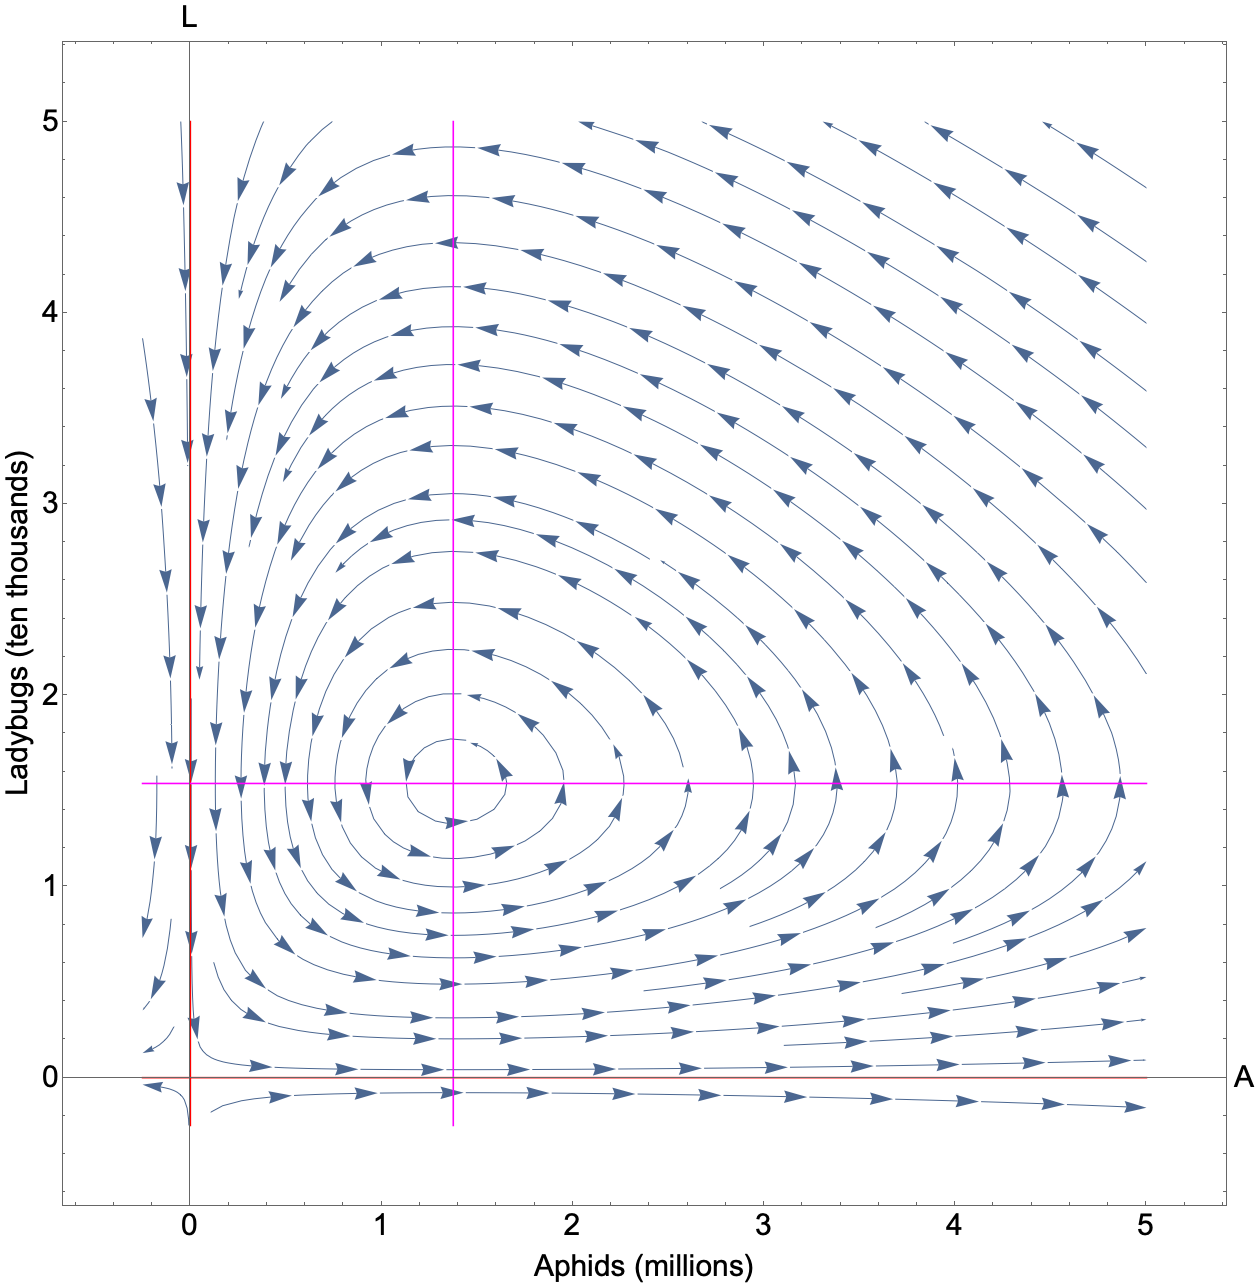
\includegraphics[width=0.45\textwidth]{pesticide_model_f1.png}
	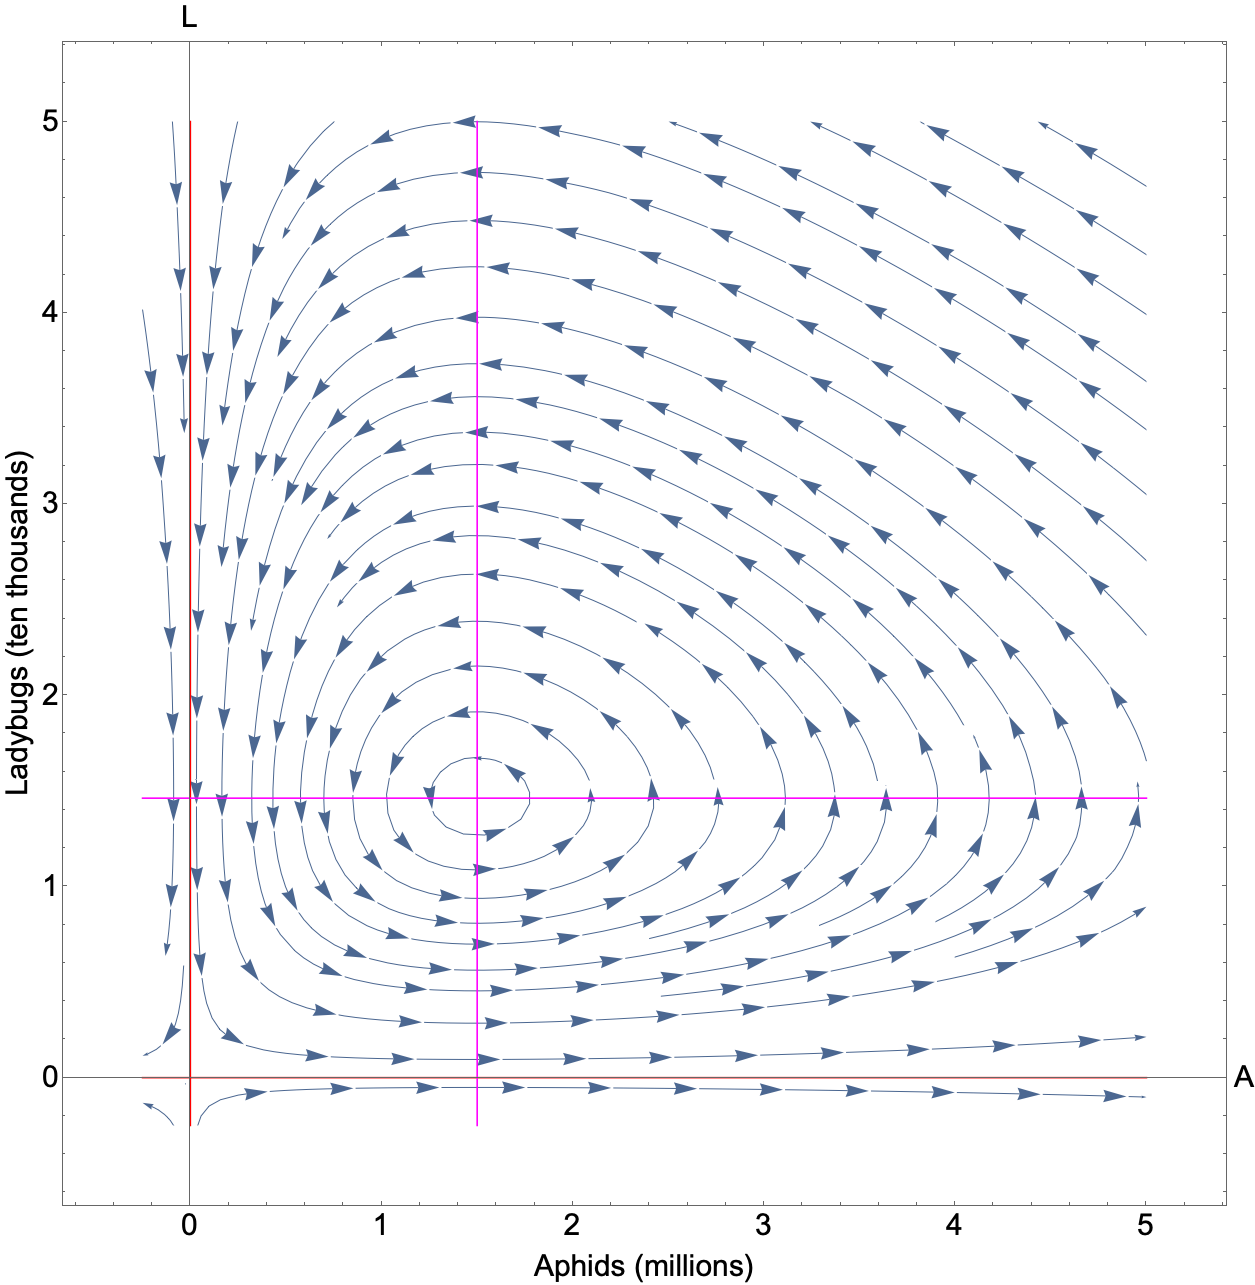
\includegraphics[width=0.45\textwidth]{pesticide_model_f2.png} \\ [1ex]
	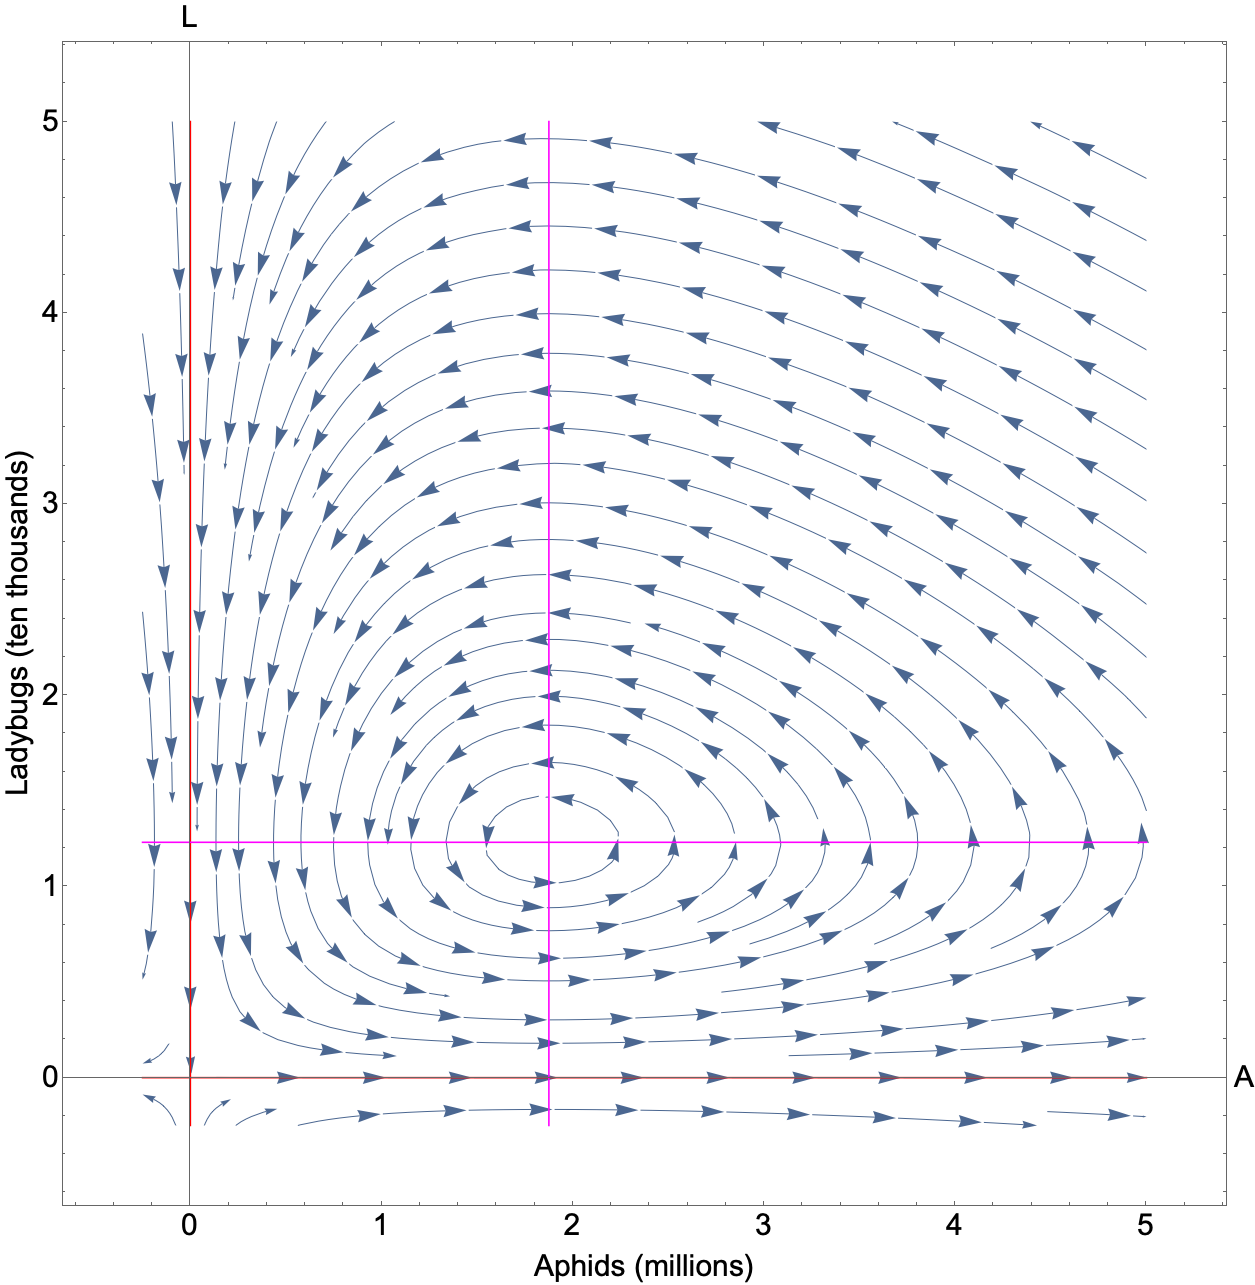
\includegraphics[width=0.45\textwidth]{pesticide_model_f3.png}
	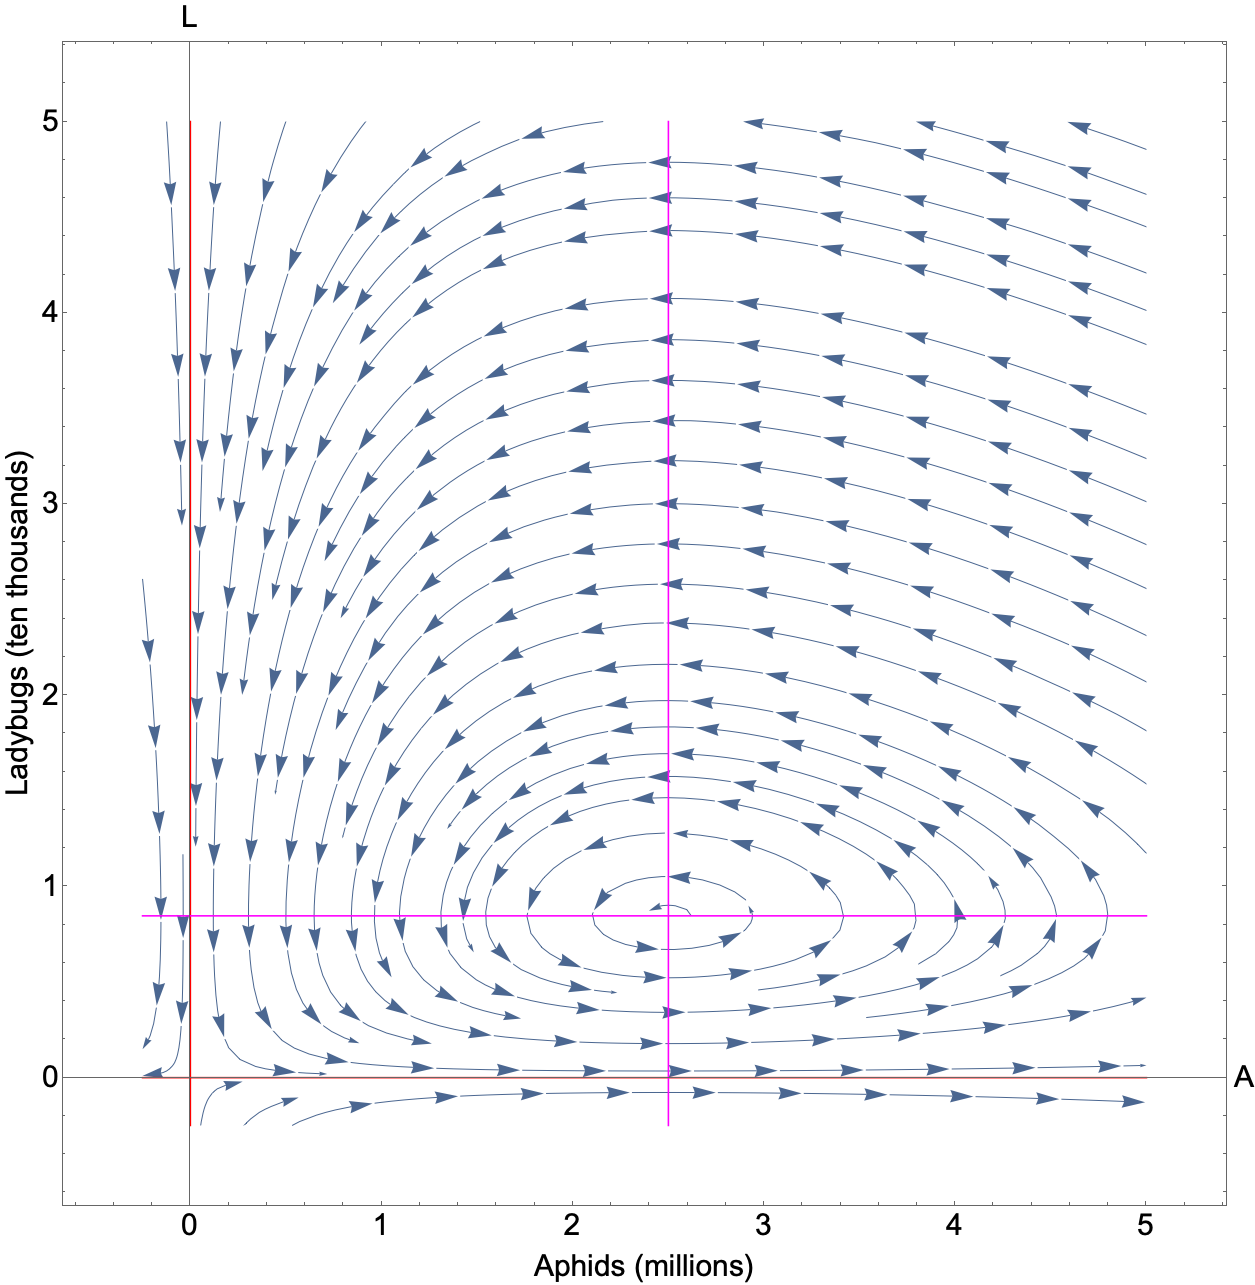
\includegraphics[width=0.45\textwidth]{pesticide_model_f4.png}
	\caption{Clockwise from top left: \( f = 0.01, \ 0.02, \ 0.05, \ 0.10 \). While the stability of the equilibria never changes, as the value of \(f\) increases, the relative population of aphids appears to increase as well, indicating that pesticides may be harmful to an IPM setup.}
	\label{fig:pesticidemodelnullcline}
\end{figure}

\np

\setcounter{tocdepth}{1}

\section{Recommendations for Pest Management}

\subsection{Recommended IPM Strategies}

Since there are currently no predators in the apple orchard, we can assume that the current population of aphids is stable at the carrying capacity. I.e., the current population of aphids will likely not grow or decline significantly. Barring any ecological disasters, introducing any population of ladybugs should decrease the population of aphids. However, the amount of ladybugs introduced will affect the amount of time needed for the populations to stabilize.

Introducing more than approximately 9,500 ladybugs (the stable value for the current population system) will cause the ladybug population to quickly decline to this value, so purchasing any more ladybugs than this amount would be a waste of money. Introducing between 8000--9000 ladybugs into the orchard should be plenty to regulate the current aphid population within a decent amount of time; less may be introduced, but less ladybugs will cause a slower decline in the aphid population.

The model used in order to understand the population dynamics between the aphids and ladybugs predicts that if any amount of ladybugs are introduced, over some period of time the orchard will be able to hold about 9,500 ladybugs and 1.25 million aphids. While 1.25 million aphids seems like a lot, it is less than half of the amount of aphids which would be sustained by the orchard if no predators were present. Regardless of the amount of aphids the orchard could support, when this value is changed in the mathematical model, we see the same result: introducing ladybugs will always lead to a stable aphid population which seems to be at most half the amount which would occur naturally if no predators were present.

Thus, introducing any amount of ladybugs would be beneficial in controlling the amount of aphids in the orchard. Introducing more than 9,500 ladybugs into the orchard will not make a difference. However, up to this limit, increasing the amount of ladybugs introduced will cause a faster decline of the aphid population. The number of ladybugs purchased for introduction into the orchard should depend on the severity of the aphid problem: if the aphids are a real nuisance, between 8--9 thousand ladybugs should be introduced, but if the aphids are merely an inconvenience, a smaller population of ladybugs will do the same job just fine.

\subsection{Recommended Use of Pesticides}

Although this may seem counter-intuitive, using pesticides alongside the IPM recommendations is not recommended. Mathematically, spraying any amount of pesticides will alter the delicate balance of the IPM system enough to cause a detrimental effect. Even if pesticides are sprayed at a low rate, the overall aphid population will increase, as aphids and ladybugs are equally affected by pesticides. As one case study, spraying pesticides at a rate which kills one percent of all insects in the orchard will have a final effect of an aphid population of approximately 1.38 million, compared to the final IPM aphid population of approximately 1.25 million aphids.

Increasing the pesticide spraying rate shows a similar effect: the smaller ladybug population is affected by the pesticides more than the aphid population, which allows the aphid population to grow to a larger equilibrium size. So, a well-intentioned application of pesticides may do more harm than good to an orchard where an IPM system is already in place.

\np

%The references (if needed) goes here.

\bibliographystyle{plain}
\bibliography{project1bib}

\end{document}